% !TeX spellcheck = en_US

\documentclass[conference]{IEEEtran}
\IEEEoverridecommandlockouts
% The preceding line is only needed to identify funding in the first footnote. If that is unneeded, please comment it out.
\usepackage{cite}
\usepackage{amsmath,amssymb,amsfonts}
\usepackage{algorithmic}
\usepackage{graphicx}
\usepackage{textcomp}
\usepackage{xcolor}
\usepackage{algorithm2e}
\def\BibTeX{{\rm B\kern-.05em{\sc i\kern-.025em b}\kern-.08em
    T\kern-.1667em\lower.7ex\hbox{E}\kern-.125emX}}
\begin{document}

\title{Applying stop words filtering and stemming for sentiment analysis}

\author{
	\IEEEauthorblockN{Abdelkrime Aries}
	\IEEEauthorblockA{%
		\textit{Ecole nationale Supérieure d'Informatique (ESI)}\\
		Algiers, Algeria \\
		ab\_aries@esi.dz
	}
%	\and
%	\IEEEauthorblockN{Abdelkrime Aries}
%	\IEEEauthorblockA{%
%		\textit{Ecole nationale Supérieure d'Informatique (ESI)}\\
%		Algiers, Algeria \\
%		ab\_aries@esi.dz
%	}

}

\maketitle

\begin{abstract}
Nowadays, sentiment analysis gained more importance among enterprises in order to collect users' opinion about their products and services. 
Using this solution in mobile applications needs a more small model.
Also, when accompanied with search engines, this solution must be fast.
To this end, we propose a new method which uses a neural network to classify sentiments.
This neural network is kept small as possible to save model's space.
In addition, we apply stop words filtering and stemming which reduces vocabulary space.
This leads to a more compact representations of texts.
Our experimentation shows that this method improves prediction time and model's size.
Although it did not improve recall and precision, it gives almost the same performance as the state of art methods with less size and time.
\end{abstract}

\begin{IEEEkeywords}
sentiment analysis, NLP, stemming, neural networks
\end{IEEEkeywords}

\section{Introduction}
Sentiment analysis gains a lot of attention in late years.
Due to its use in collecting users' sentiment about a given subject, it became a preferred solution to many enterprises and even governments.
The later uses it in order to get an idea about citizens views to certain political issues.

\section{Related works}

In this section, we will present two main approaches to sentiment analysis.
The two of them are widely used till nowadays.

\subsection{Rule-based methods}

In \cite{18-bettiche-al}, the authors proposed two methods where one of them is rule based.
They annotated some words as positive or negative.
Then they used Levenstein to predict if two words are similar in term of characters. 
Each sentence is scored based on the words it contains.

\subsection{ML-based methods}

The other method of \cite{18-bettiche-al} can be describe as feeding the scores of the words into a machine learning algorithm to classify the sentiment.
Another similar work is that of \cite{18-guellil-al}.
In this work, the polarity of each word is not represented as 1 or -1, but rather a score.

\section{Method overview}

Our method have three phases: preprocessing, sentence representation and classification.
These phases are executed in a sequential fashion as represented in Figure \ref{fig:method}.
\begin{figure}[htbp]
\centerline{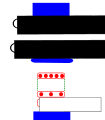
\includegraphics[width=.2\textwidth]{img/method.pdf}}
\caption{Method overview}
\label{fig:method}
\end{figure}

\subsection{Preprocessing}

In preprocessing phase, we use three tasks: tokenization, stemming and stop-words removal. 
The used tools are shown in Table \ref{tab:preprocess}. 
First, we tokenize each sentence using a personalized method based only on regular expressions.
We noticed that existing tokenizers tend to over-complicate the task.
This is why we use blanks to separate tokens in such manner: \textbf{r'(?u)\textbackslash b\textbackslash w\textbackslash w+\textbackslash b'}.

The next task is stop-words removal.
It is very important to our method since these words usually do not carry any sentiment whatsoever.
Also, they clutter the representation with unnecessary space.

Stemming is another task which helps freeing more representation space.
Words like "do", "doer", "doing", "done" each is represented as a feature in representation vector.
When stemmed, all these words will be "do" resulting in one feature instead of four. 
This will result in less vocabulary and hence less representation space.

\begin{table}[htbp]
\caption{Preprocessing tasks}
\begin{center}
\begin{tabular}{ll}
\hline\hline
\textbf{Task} & \textbf{Tool}  \\
\hline
Tokenization & RegExp \\
Stemming & Porter stemmer (NLTK) \\
Stop-words filtering & NLTK \\
\hline\hline
\end{tabular}
\label{tab:preprocess}
\end{center}
\end{table}

Theses tasks are ordered as follows: tokenization, stop-words filtering then stemming.
They are not executed in a sequential fashion.
Instead, there is some overlap between them.
The process can be better understood consulting Algorithm \ref{algo:preprocess}.

\begin{algorithm}[ht]
	\KwData{a sentence}
	\KwResult{a list of tokens}
	create an empty list\;
	tokenize sentence\;
	\ForEach{word in tokenized sentence}{
		\If{word not in stop words}{
			stem the word\;
			add the stem to the list\;
		}
	}
	\caption{Preprocessing pipeline}
	\label{algo:preprocess}
\end{algorithm}

\subsection{Sentence representation}

To represent a sentence, we use \textit{Term Frequency (TF)}. 
The problem with this representation is that it takes more space with a large vocabulary.
Sometimes, it would be better if some words are scarified in order to free more space. 
To demonstrate how this representation works, lets take these two sentences:
\begin{itemize}
	\item The sky is clear today
	\item A cloudy sky is not a clear sky
\end{itemize}

There are different words assuming we transform them into lowercase: "a", "clear", "cloudy", "is", "not", "sky", "the", "today".
The first sentence will be encoded as: [0, 1, 0, 1, 0, 1, 1, 1] following the same order of these words.
The second will have the vector [2, 1, 1, 1, 1, 2, 0, 0] as representation.
TF is representation simple to generate, it represents sentences directly and it is numeric.
This makes it an adequate representation for neural networks input.

\subsection{Classification}

To classify a text, we use a simple multi-layer perceptron (MLE). 
We assume the input $x$ is sentence representation and $\hat{y}$ is a three values vector representing the output class.
We used a hidden layer with a ReLu activation function as shown in equation \ref{eq:firestlayer}.
$W_h$ and $b_h$ are the parameters to be trained.
\begin{equation}
	h = ReLu(W_h . x + b_h)
	\label{eq:firestlayer}
\end{equation}
The output layer contains three neurons; the same number as classes.
It is formulated as illustrated in equation \ref{eq:lastlayer}.
\begin{equation}
	\hat{y} = Softmax(W_o . h + b_o)
	\label{eq:lastlayer}
\end{equation}

To train this model, we used categorical cross-entropy as loss function.
Assuming the input samples size is $M$ and $y$ are their real classes, this loss is expressed in equation \ref{eq:loss}.
\begin{equation}
	J(W, b) = - \sum\limits_{i=1}^M y_i \log(\hat{y}_i)
	\label{eq:loss}
\end{equation}

\section{Experiments}

\subsection{Metrics}

To test our method, we use recall and precision expressed in equation \ref{eq:rp}.
\begin{equation}
	R = \frac{TP}{TP + FN} \hspace{24pt} P = \frac{TP}{TP + FP}
	\label{eq:rp}
\end{equation}
Where TP, TN, FP and FN mean true positives, true negatives, false positives, and false negatives respectively.
In addition, we use prediction time to compare different systems.

\subsection{Data preparation}

We used "Financial sentiment analysis" dataset.
There are 5842 samples of which 1852 are positive, 3130 are neutral and 860 are negative.
We split this dataset into two: training (70\%) and test (30\%).

We generated sentences representations without any processing other than tokenization and normalization. 
To test with our pretraining, we generated another representation with a limited predefined vocabulary size (3000).
A third representation is generated as the second but without vocabulary limit.

\subsection{Baseline}

The baseline system uses the same architecture as ours.
But, it takes all tokens in consideration; no stemming or stop-words filtering.

\subsection{Training}

We trained three models using the previous representations.
Table \ref{tab:train} represents P, R and time for the three models.
We used the micro-average since it is immune to unbalanced lasses.
This allows us to compare the convergence of these models: how well they can represent the training dataset.

\begin{table}[htbp]
	\caption{Performance in training dataset}
	\begin{center}
		\begin{tabular}{lll}
			\hline\hline
			\textbf{Model} & \textbf{P} & \textbf{R}\\
			\hline
			Our method           & \textbf{0.94} & 0.89 \\
			Our method (limited) & 0.92 & 0.86 \\
			\hline
			Baseline             & \textbf{0.94} & \textbf{0.93} \\
			\hline\hline
		\end{tabular}
		\label{tab:train}
	\end{center}
\end{table}

We can note that the baseline and our method without vocabulary size limitation converge better.
This is understandable since more information means more ways to represent a solution.
 

\subsection{Test}

Like in training phase, we will test recall and precision of each model.
This time, they will be tested on a new dataset, where the vocabulary can be different.
In addition to these metrics, we use prediction time.
Table \ref{tab:test} represents test performance for the three models.

\begin{table}[htbp]
	\caption{Performance in test dataset}
	\begin{center}
		\begin{tabular}{llll}
			\hline\hline
			\textbf{Model} & \textbf{P} & \textbf{R} & \textbf{time (ms)} \\
			\hline
			Our method           & 0.68 & 0.60 & 0.001302\\
			Our method (limited) & 0.68 & 0.59 & \textbf{0.001006} \\
			\hline
			Baseline             & \textbf{0.69} & \textbf{0.61} & 0.007595 \\
			\hline\hline
		\end{tabular}
		\label{tab:test}
	\end{center}
\end{table}

Although our method is not as good as te baseline, it still too close in term of recall and precision.
As for the prediction time, it is way better.
Even if we sacrifice a little in term of classification capacity, we enormously gained in term of prediction time.

\section{Conclusion}

In this paper, we proposed a method to enhance sentiment analysis in term of prediction time.
Our aim is to use this model with a research engine.
This is why prediction time is very important.
Even if we sacrifice other aspects of performance, the aspect of time must be the first priority.

Our method show promising results since we could ameliorate model space and prediction time.
Other improvements can be done such as exploring other methods of sentence and word representation.
Also, experimenting with different classification algorithms can be beneficial.

%\section*{Acknowledgment}
%
%The preferred spelling of the word ``acknowledgment'' in America is without 
%an ``e'' after the ``g''. Avoid the stilted expression ``one of us (R. B. 
%G.) thanks $\ldots$''. Instead, try ``R. B. G. thanks$\ldots$''. Put sponsor 
%acknowledgments in the unnumbered footnote on the first page.

\section*{References}

\bibliographystyle{IEEEtran}
\bibliography{biblio}

\end{document}
